%% ------------------------------------------------------------------- %%
%% ------------------------------------------------------------------- %%
%% ------------------------------------------------------------------- %%
%% ------------------------------------------------------------------- %%
\chapter{Propuesta}
\label{cap:propuesta}

\lhead{\emph{Propuesta}} 
%% ------------------------------------------------------------------- %%
%% ------------------------------------------------------------------- %%
%% ------------------------------------------------------------------- %%
%% ------------------------------------------------------------------- %%
%% ------------------------------------------------------------------- %%
%% ------------------------------------------------------------------- %%

%% -------------------------------------------------------------------- %%
%% -------------------------------------------------------------------- %%


En este capítulo presetaremos la propuesta y como se relaciona con los métodos tradicionales de detección de neo antígenos.

\section{Detección de neo antígenos (\textit{pipeline})}

Según \cite{gopanenko2020main}, la detección de neo antígenos podría clasificarse en tres grupos: (1) basados en genómica, (2) basados en \textit{Mass Spectrometry} (MS) y (3) basados en estructura. \\

La detección de neo antígenos basada en genómica sigue un proceso muy largo e involucra muchas herramientas, debido a esto se han propuesto bastantes \textit{pipelines}. El proceso general consta de varias etapas presentadas en la Figura \ref{fig:neo_det_seq}, a continuación detallaremos cada una de ellas y explicaremos en qué fase se ubica la propuesta de esta tesis:

\begin{enumerate}
	\item \textbf{Secuenciamiento}. La primera fase consiste en el secuenciamiento de DNA, en este caso se toman muestras de sangre al tener menos riesgo de no ser contaminadas por un tumor \citep{borden2022cancer}. Para la secuenciación, se puede obtar por \textit{Whole Genome Sequencing} (WGS) o \textit{Whole Exome Sequencing} (WES), la primera tiene la ventaja de tener mucha más información de mutaciones pero es muy costoso. Esta fase, también puede retroalimentarse con secuenciamiento de RNA (seqRNA). Una tendencia reciente fomenta el uso de \textit{RiboSeq}, este tiene la ventaja de tener más información de las proteínas formadas en los Ribosomas, lamentablemente no se tienen muchas muestras \citep{borden2022cancer}.
	
	\item \textbf{Alineamiento y procesamiento}. En esta fase, se evalúa la calidad del secuenciamiento, se elimina el ruido y se realiza un alineamiento con un genoma base. Como resultado se obtienen archivos BAM (resultado del alineamiento) y FastQC (calidad de cada secuenciación).
	
	\item \textbf{Identificación de neo antígenos}. En esta fase se analiza las mutaciones de la secuencia, generalmente se obtienen \textit{Variant Calling Files} (VCF). En esta etapa, es importante secuenciar las proteínas \textit{Human Leukocyte Antigens} (HLA), estas representan las proteínas MHC mencionadas anteriormente. Luego con información del tipo de HLA y mutaciones, se puede identificar los posibles neo antígenos. Esta fase puede ser retroalimentada de \textit{RiboSeq} y datos de MS.
	
	\begin{figure}[H]
		\centering
		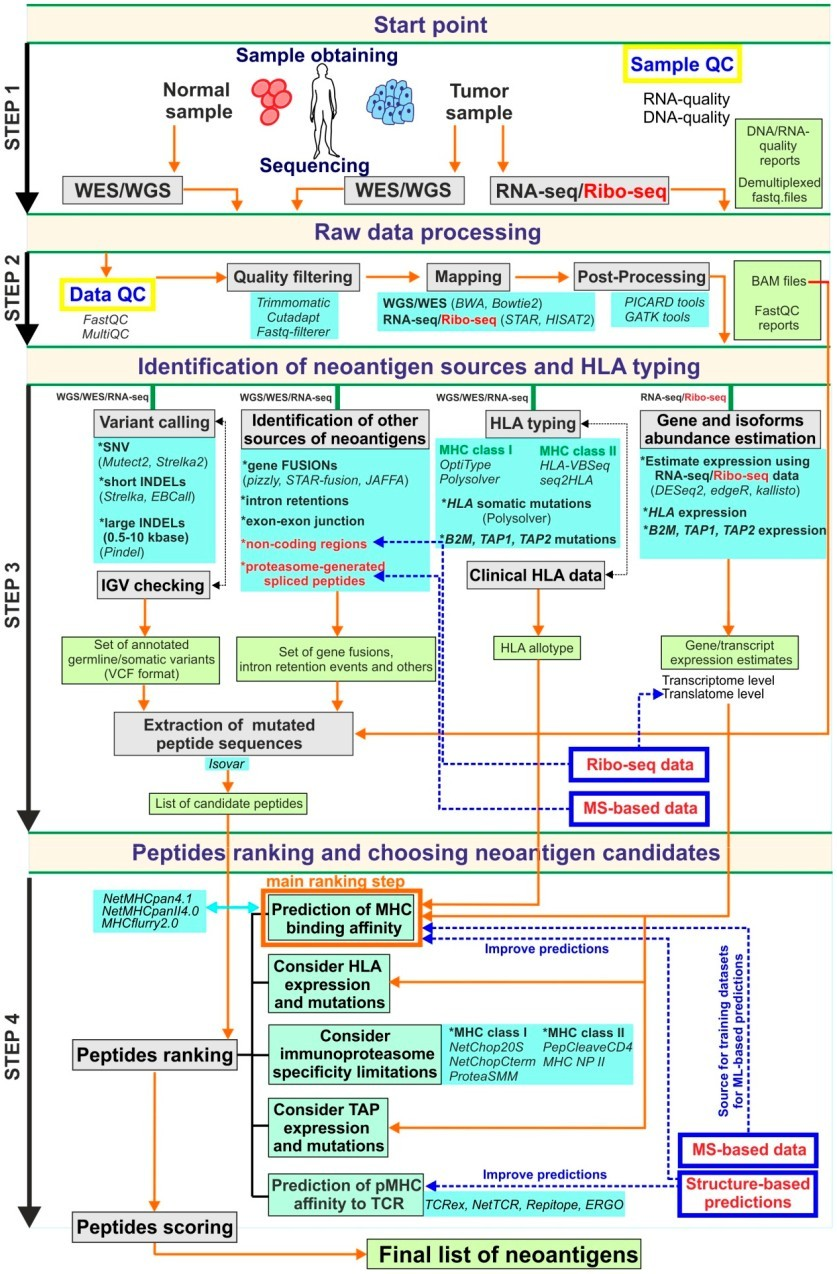
\includegraphics[width=0.9\textwidth]{img/neoantigen/method}	
		\caption{Proceso general utilizado para la detección de neo antígenos a partir de secuencias de DNA. Fuente: \cite{gopanenko2020main}.}
		\label{fig:neo_det_seq}
	\end{figure}
	
	\item \textbf{Priorización de neo antígenos}. En esta fase se filtran los neo antígenos identificados anteriormente. Este problema es conocido mayormente como: \textit{MHC-peptide binding}, en este caso se predice el enlace entre el neo antígeno y la proteína MHC \textbf{(la propuesta de la tesis se enfoca en esta etapa)}. Las herramientas con mejor desempeño son \textit{NetMHCpan4.1} y \textit{MHCflurry2.0} según varios \textit{benchmarkings} \citep{bonsack2019performance, zhao2018systematically, paul2020benchmarking, trolle2015automated}. Recientemente una nueva propuesta ha superado a \textit{NetMHCpan4.1}, esta propuesta obtuvo buenos resultados utilizando  \textit{protein language models} \citep{hashemi2022improved}. Finalmente, se predice la afinidad de T-Cell Receptor (TCR) con pMHC (peptide-MHC binding).
\end{enumerate}


Recientemente, se está utilizando otros enfoques para mejorar la detección de neo antígenos, por ejemplo, se puede utilizar datos MS para mejorar la identificación de neo antígenos. Luego, el enfoque basado en estructura que utiliza información de propiedades químicas y físicas de los péptidos puede ser utilizada para mejorar la predicción de afinidad TCR y pMHC \citep{borden2022cancer, gopanenko2020main}.\\


\section{Predicción de la afinidad peptido-MHC (peptide-MHC binding)}

La propuesta se inspira en los trabajos de \cite{cheng2021bertmhc} y \cite{hashemi2022improved}. Ambos proponen el uso de \textit{transfer  learning} a partir de los modelos pre-entrenados BERT \citep{devlin2018bert} y ESM-1b \citep{rives2021biological} respectivamente. \\


El modelo \textit{Bidirectional Encoder Representations from Transformers.} (BERT), fue diseñado para el pre-entrenamiento de representaciones bidireccionales de textos no etiquetados. Este modelo fue diseñado inicialmente para el procesamiento natural del lenguaje, pero en el trabajo de \cite{rao2019evaluating}, se planteó su uso para secuencias de aminoácidos. Es así que \cite{rao2019evaluating} entrenan BERT con 31 millones de secuencias de proteínas y llaman a su propuesta \textit{Tasks Assessing Protein Embeddings} (TAPE).\\

Recientemente, Facebook desarrolla el modelo ESM-1b \citep{rives2021biological}. La propuesta se basa en el modelo RoBERTa \citep{liu2019roberta}, la cuál es una optimización de BERT. Luego, ESM-1b fue entrenado con la base de datos Uniref50 \citep{suzek2015uniref}, esta base de datos cuenta con aproximadamente 250 millones de secuencias de proteínas. En este caso, se realizó un entrenamiento no supervisado, se ocultaron las etiquetas referentes a la estructura o función de las proteínas.\\

Entonces, la propuesta de la tesis se basa en utilizar \textit{transfer learning} del modelo pre-entrenado ESM-1b, luego se va a utilizar otra red neuronal paralela que se alimente de datos físico-químicos de los aminoácidos. Se propone utilizar las propiedades físico-químicas de los aminoácidos, porque en varios ensayos clínicos se ha comprobado que influyen en la predicción \textit{peptide-MHC binding} y \textit{pMHC-TCR presentation} \citep{gopanenko2020main, borden2022cancer}. Luego, las dos redes neuronales paralelas se unirán en una red neuronal totalmente conectada (ver Figura \ref{fig:proposal}). El objetivo, es aprovechar las propiedades físico-químicas de los aminoácidos para mejorar la afinidad \textit{peptide-MHC}.




\begin{figure}[H]
	\centering
	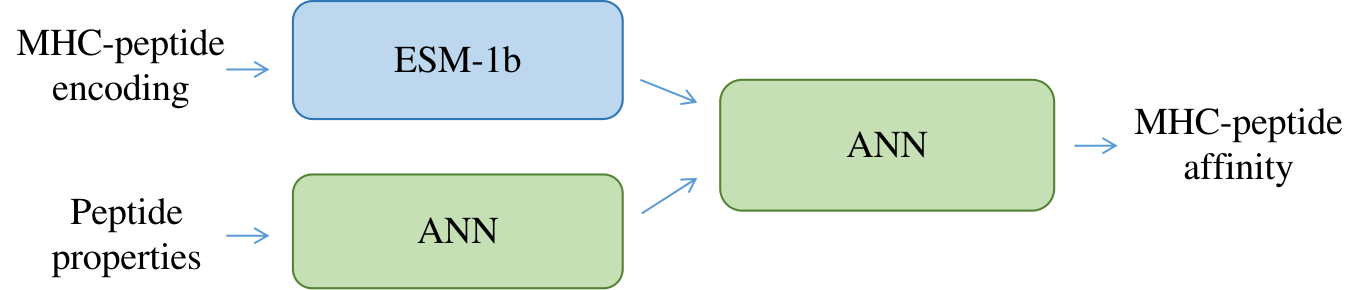
\includegraphics[width=0.8\textwidth]{img/neoantigen/proposal}	
	\caption{Propuesta de \textit{transfer learning} de ESM-1b y una red neuronal paralela para la predicción de la afinidad entre un péptido y MHC (peptide MHC binding).}
	\label{fig:proposal}
\end{figure}


Para los entrenamientos y experimentos se utilizará la base de datos HLA3D \citep{li2022hla3d}, esta contiene información de 1296 aminoácidos. Luego, también utilizaremos las muestras recolectadas de \cite{hashemi2022improved}.

